\documentclass[12pt, a4paper]{report}
\usepackage[top=1cm, left=0.8cm, right=0.8cm]{geometry}

\usepackage[utf8]{inputenc}
\usepackage[russian]{babel}

\usepackage{array}
\newcolumntype{M}[1]{>{\centering\arraybackslash}m{#1}}

\usepackage{hyperref}
\hypersetup{
	colorlinks,
	citecolor=black,
	filecolor=black,
	linkcolor=black,
	urlcolor=black
}

\usepackage{sectsty}
\allsectionsfont{\centering}

\usepackage{indentfirst}
\setlength\parindent{24pt}
 
\usepackage{listings}
\usepackage{xcolor}
\definecolor{codegreen}{rgb}{0,0.6,0}
\definecolor{codegray}{rgb}{0.5,0.5,0.5}
\definecolor{codepurple}{rgb}{0.58,0,0.82}
\definecolor{backcolour}{rgb}{0.95,0.95,0.92}
\lstdefinestyle{mystyle}{
    backgroundcolor=\color{backcolour},
    commentstyle=\color{codegreen},
    keywordstyle=\color{magenta},
    numberstyle=\normalsize\color{codegray},
    stringstyle=\color{codepurple},
    basicstyle=\ttfamily\footnotesize,
    breakatwhitespace=false,
    breaklines=true,
    captionpos=b,
    keepspaces=true,
    numbers=left,
    numbersep=5pt,
    showspaces=false,
    showstringspaces=false,
    showtabs=false,
    tabsize=2
}

\usepackage{graphicx}
\graphicspath{{assets/}}

\begin{document}
	\begin{titlepage}
			\begin{center}
				\large \textbf{Министерство науки и высшего образования Российской Федерации} \\
				\large \textbf{Федеральное государственное бюджетное образовательное учреждение высшего образования} \\
				\large \textbf{«Российский химико-технологический университет имени Д.И. Менделеева»} \\

				\vspace*{4cm}
				\LARGE \textbf{ОТЧЕТ ПО ЛАБОРАТОРНОЙ РАБОТЕ №3}

				\vspace*{4cm}
				\begin{flushright}
					\Large
					\begin{tabular}{>{\raggedleft\arraybackslash}p{8.85cm} p{10.8cm}}
						Выполнил студент группы КС-36: & Золотухин Андрей Александрович \\
						Ссылка на репозиторий: & https://github.com/ \\ 
						& CorgiPuppy/ \\
						& info-sys-admin-labs \\
						Принял: & Митричев Иван Игоревич \\
						Дата сдачи: & 26.02.2025 \\
					\end{tabular}

				\end{flushright}

				\vspace*{6cm}
				\Large \textbf{Москва \\ 2025}
			\end{center}
		\end{titlepage}
		
		\tableofcontents	
		\thispagestyle{empty}
		\newpage

		\pagenumbering{arabic}
		
		\section*{Описание и выполнение задачи}
		\addcontentsline{toc}{section}{Описание и выполнение задачи}	
		\large
		Задания 1-21 выполняются в терминале (bash) со скриншотами. \par

			\subsection*{Задание 1}
			\addcontentsline{toc}{subsection}{Задание 1}	
			Создайте \underline{3} текстовых файла с помощью команд \textbf{touch}, \textbf{>}, \textbf{nano}. В каждом файла должно быть по \underline{2} строки текста.
			\lstset{style=mystyle}
			\lstinputlisting[language=Bash]{src/task1/main.sh}
			\begin{center}
				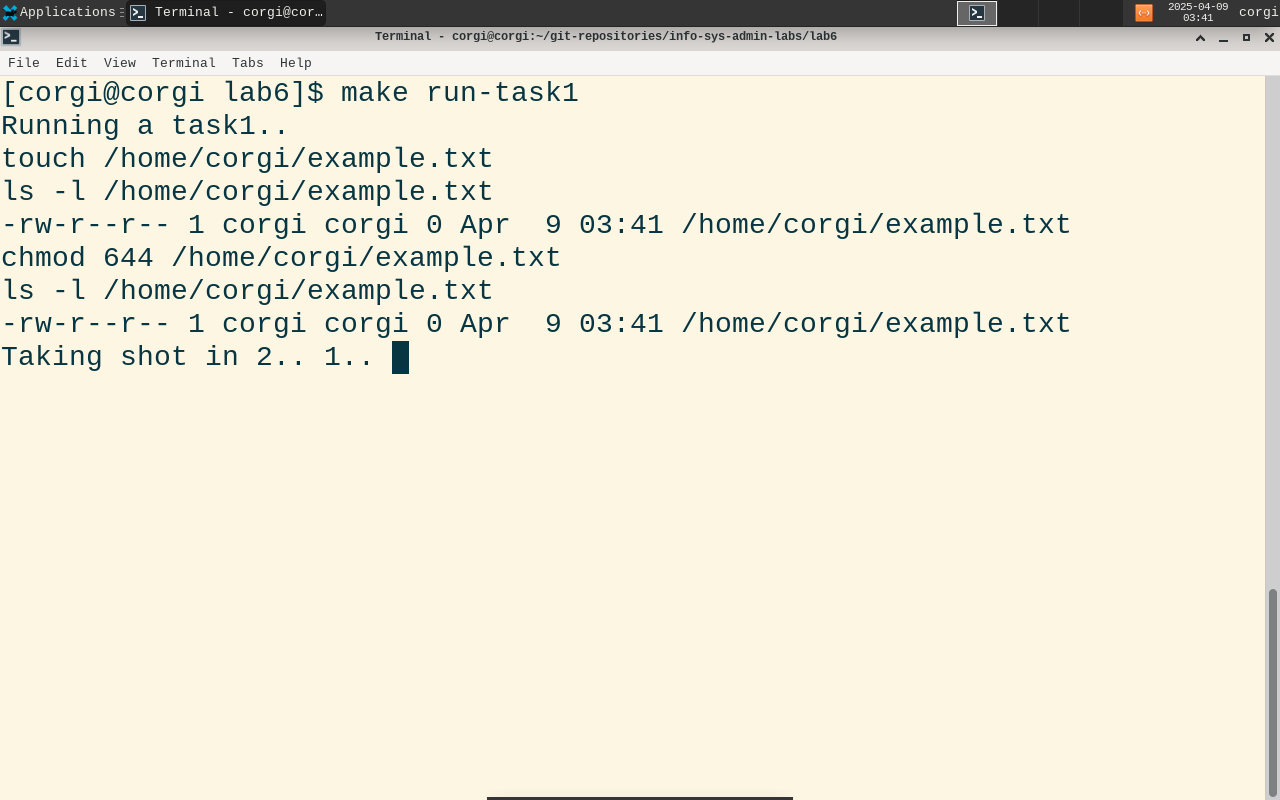
\includegraphics[width=500pt]{task1.png}
			\end{center}

			\subsection*{Задание 2}
			\addcontentsline{toc}{subsection}{Задание 2}
			Удалите один из файлов командой.
			\lstset{style=mystyle}
			\lstinputlisting[language=Bash]{src/task2/main.sh}
			\begin{center}
				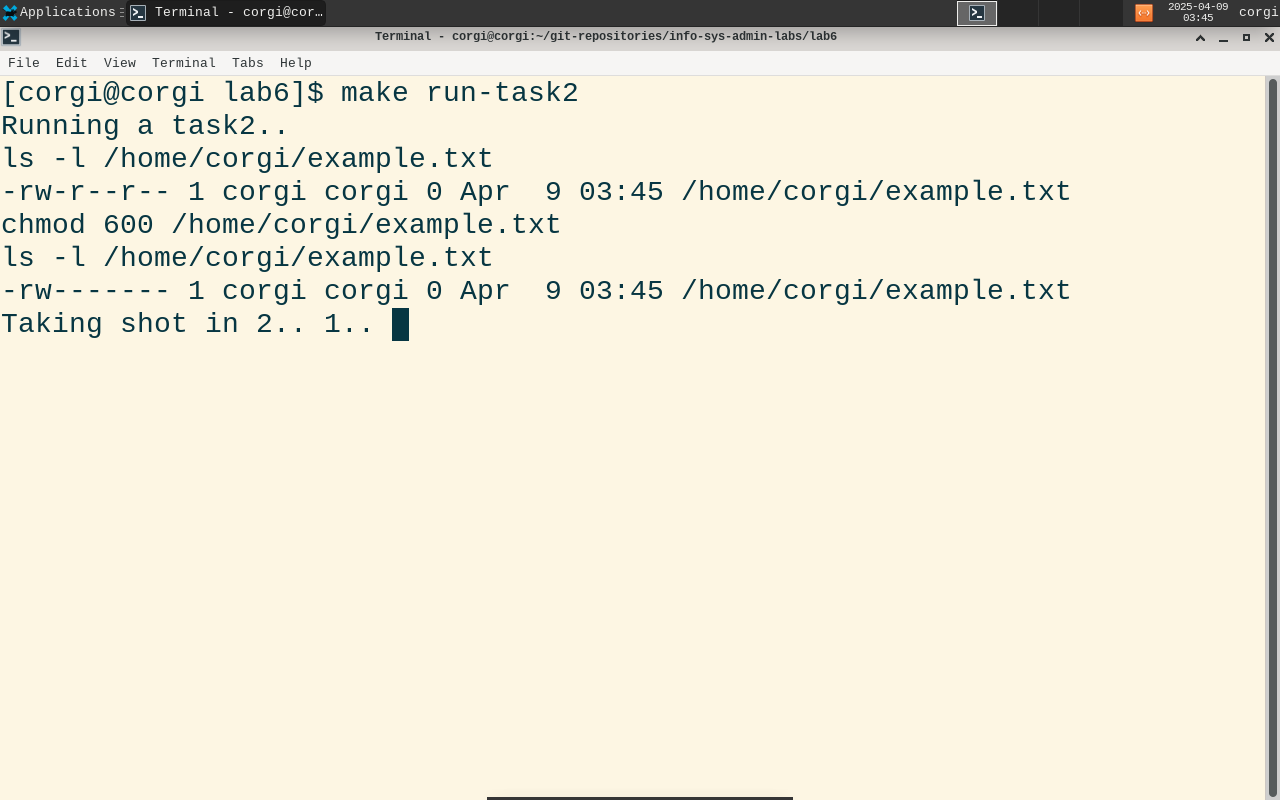
\includegraphics[width=500pt]{task2.png}
			\end{center}

			\subsection*{Задание 3}
			\addcontentsline{toc}{subsection}{Задание 3}
 			Передайте один из файлов во владение пользователю \textit{root}. Поменяйте права на этот файл на \underline{700}.
			\lstset{style=mystyle}
			\lstinputlisting[language=Bash]{src/task3/main.sh}
			\begin{center}
				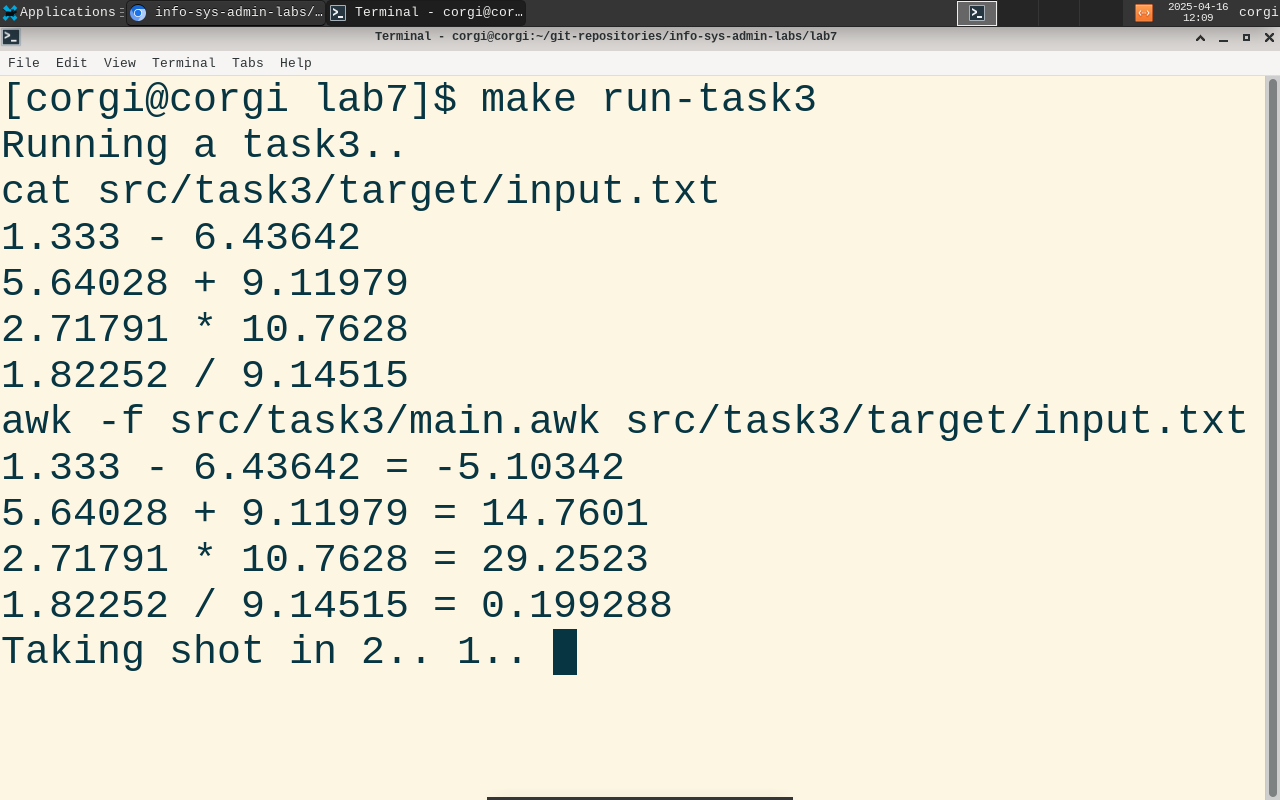
\includegraphics[width=500pt]{task3.png}
			\end{center}
			
			\subsection*{Задание 4}
			\addcontentsline{toc}{subsection}{Задание 4}
			Попытайтесь из-под вашего обычного пользователя удалить предыдущий файл, на вопрос отвечайте \textit{«Нет»}. Попытайтесь с опцией \textbf{-f}.
			\lstset{style=mystyle}
			\lstinputlisting[language=Bash]{src/task4/main.sh}
			\begin{center}
				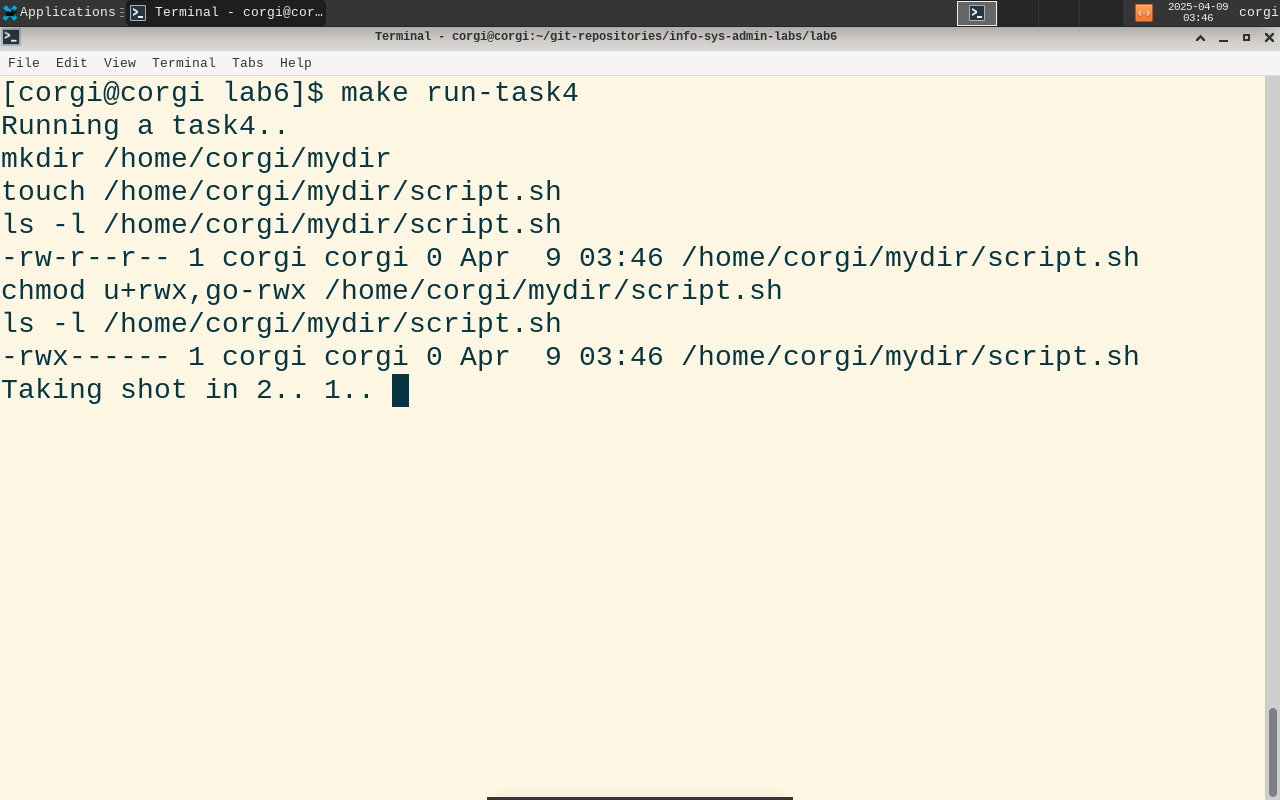
\includegraphics[width=500pt]{task4.png}
			\end{center}
	
			\subsection*{Задание 5}
			\addcontentsline{toc}{subsection}{Задание 5}
			Переименуйте третий файл в \textit{djan.conf}.
			\lstset{style=mystyle}
			\lstinputlisting[language=Bash]{src/task5/main.sh}
			\begin{center}
				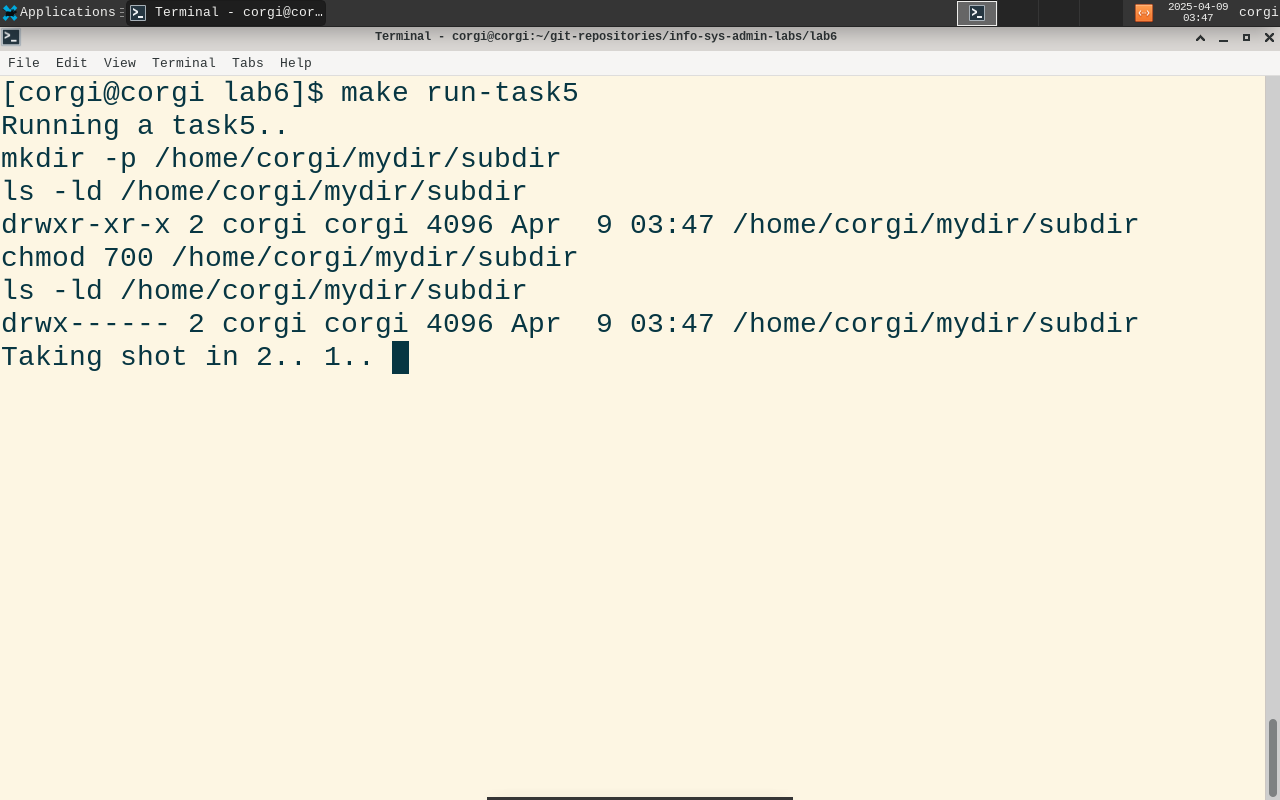
\includegraphics[width=500pt]{task5.png}
			\end{center}
	
			\subsection*{Задание 6}
			\addcontentsline{toc}{subsection}{Задание 6}
			Переместите \textit{djan.conf} в \textit{/usr/share}. Добейтесь этого.
			\lstset{style=mystyle}
			\lstinputlisting[language=Bash]{src/task6/main.sh}
			\begin{center}
				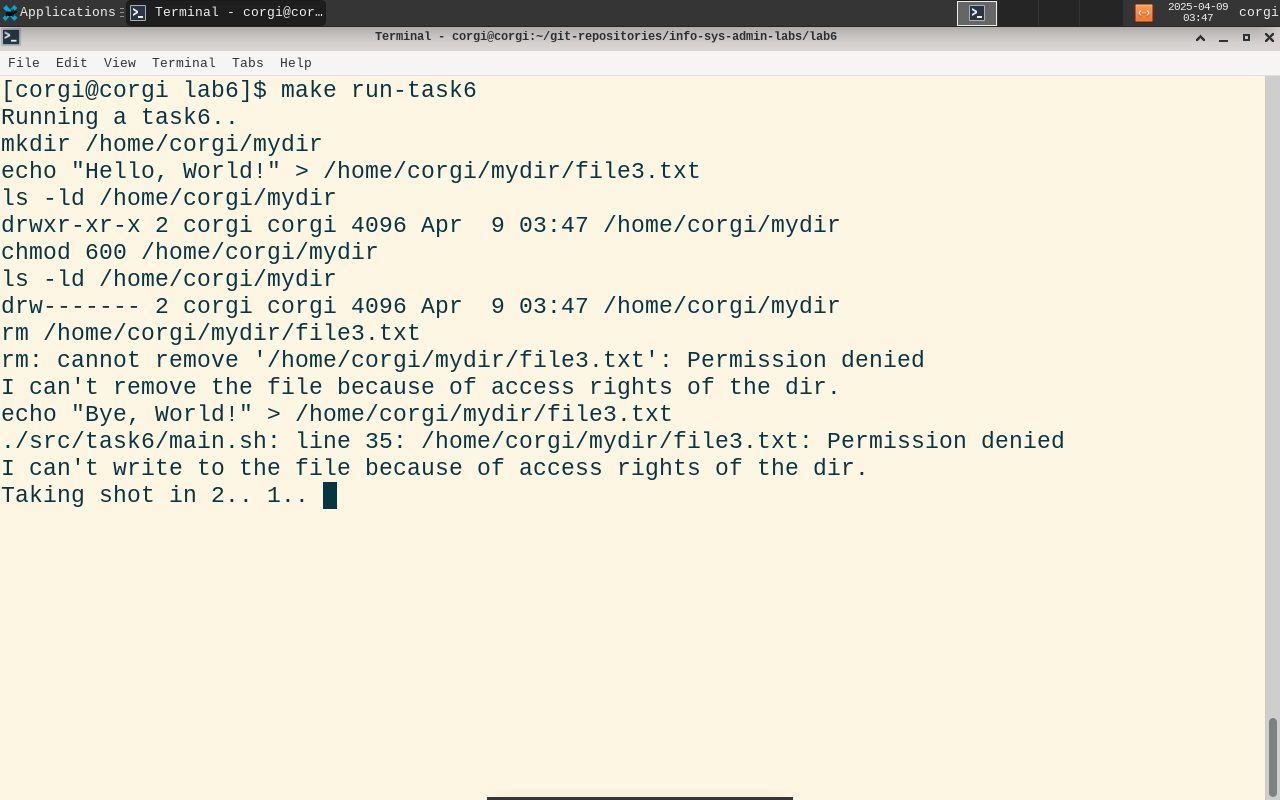
\includegraphics[width=500pt]{task6.png}
			\end{center}
	
			\subsection*{Задание 7}
			\addcontentsline{toc}{subsection}{Задание 7}
			Сделайте \textit{djan.conf} скрытым, изменив имя.
			\lstset{style=mystyle}
			\lstinputlisting[language=Bash]{src/task7/main.sh}
			\begin{center}
				\includegraphics[width=500pt]{task7.png}
			\end{center}
	
			\subsection*{Задание 8}
			\addcontentsline{toc}{subsection}{Задание 8}
			Перейдите в домашнюю папку. С помощью \textbf{ls -la} обнаружьте предыдущий файл, не переходя в директорию \textit{/usr/share}.
			\lstset{style=mystyle}
			\lstinputlisting[language=Bash]{src/task8/main.sh}
			\begin{center}
				\includegraphics[width=500pt]{task8.png}
			\end{center}
	
			\subsection*{Задание 9}
			\addcontentsline{toc}{subsection}{Задание 9}
			Изучите, что делает команда \textbf{cd -}.
			\lstset{style=mystyle}
			\lstinputlisting[language=Bash]{src/task9/main.sh}
			\begin{center}
				\includegraphics[width=500pt]{task9.png}
			\end{center}
	
			\subsection*{Задание 10}
			\addcontentsline{toc}{subsection}{Задание 10}
			Изучите, что делает нажатие TAB, стрелочки вверх и вниз на клавиатуре, а также нажатие Ctrl-r и ввод текста (введите \textbf{ls}). Возьмите на вооружение. \par
			\textit{TAB} используется для автодополнения команд или имён файлов или директорий. Например, я прописываю команду \textbf{ls} и после пробела нажимаю на \textit{TAB}, но ничего не происходит, поскольку нет одного единственного автодополнения. После второго нажатия на \textit{TAB} терминал покажет список всех доступных вариантов.
			\begin{center}
				\includegraphics[width=400pt]{task10/task10_1.png}
				\includegraphics[width=400pt]{task10/task10_2.png}
			\end{center} \par
			Если я начну вводитьимя файла или директории и нажму \textit{TAB}, терминал попытается дополнить его автоматически, поскольку существует только одно совпадение.
			\begin{center}
				\includegraphics[width=400pt]{task10/task10_3.png}
				\includegraphics[width=400pt]{task10/task10_4.png}
			\end{center} \par
			\textit{Стрелочки вверх и вниз} позволяют перемещаться по истории команд в командной строке. Например, нажатие стрелки вверх дважды покажет предпоследнюю введённую команду.	
			\begin{center}
				\includegraphics[width=400pt]{task10/task10_5.png}
				\includegraphics[width=400pt]{task10/task10_6.png}
			\end{center} \par
			А стрелка вниз - следующую после команды, к которой пришли стрелкой вверх. Это удобно для быстроого повторного ввода команд без необходимости их повторого набора.
			\begin{center}
				\includegraphics[width=400pt]{task10/task10_7.png}
			\end{center} \par
			\textit{Ctrl+R} позволяет открыть режим поиска по истории команд. Например, после ввода текста, терминал будет показывать последие команды, которые содержат введённый текст, что позволяет быстро находить и повторно использовать ранее введенные команды.
			\begin{center}
				\includegraphics[width=400pt]{task10/task10_8.png}
				\includegraphics[width=400pt]{task10/task10_9.png}
			\end{center} \par
			\textit{Ввод текста}, например, \textbf{ls} позволяет отображать список файлов и директорий в текущем каталоге. После ввода команды терминал выведет результат на экран.
			\begin{center}
				\includegraphics[width=400pt]{task10/task10_10.png}
			\end{center}

			\subsection*{Задание 11}
			\addcontentsline{toc}{subsection}{Задание 11}
			Изучите назначение файла \textit{/etc/sudoers}. Используя visudo, добавьте в файл \textit{sudoers} строку, которая позволяет пользователю \textit{student} выполнять команду \textbf{pacman} (работа с ПО).
			\begin{center}
				\includegraphics[width=500pt]{task11/task11_1.png}
				\includegraphics[width=500pt]{task11/task11_2.png}
			\end{center}
	
			\subsection*{Задание 12}
			\addcontentsline{toc}{subsection}{Задание 12}
			Добавьте пользователя \textit{student}, группа \textit{student} в операционную систему одной командой (читать \textbf{man useradd} или adduser). Зайдите под его учётной записью. Установите программу gnuplot.
			\lstset{style=mystyle}
			\lstinputlisting[language=Bash]{src/task12/main.sh}
			\begin{center}
				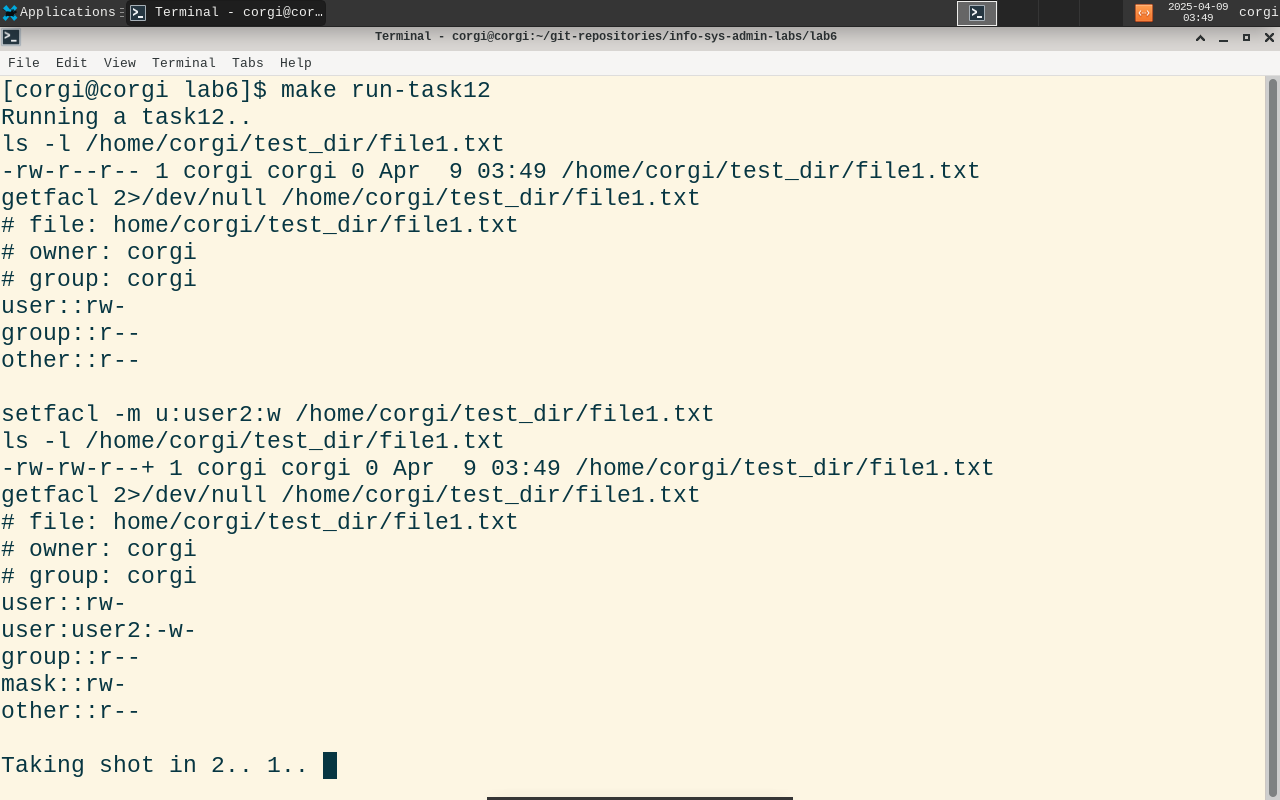
\includegraphics[width=500pt]{task12.png}
			\end{center}

			\subsection*{Задание 13}
			\addcontentsline{toc}{subsection}{Задание 13}
			Под учётной записью \textit{student} создайте командой папку \textit{PAPKA1} в директории \textit{/tmp}.
			\lstset{style=mystyle}
			\lstinputlisting[language=Bash]{src/task13/main.sh}
			\begin{center}
				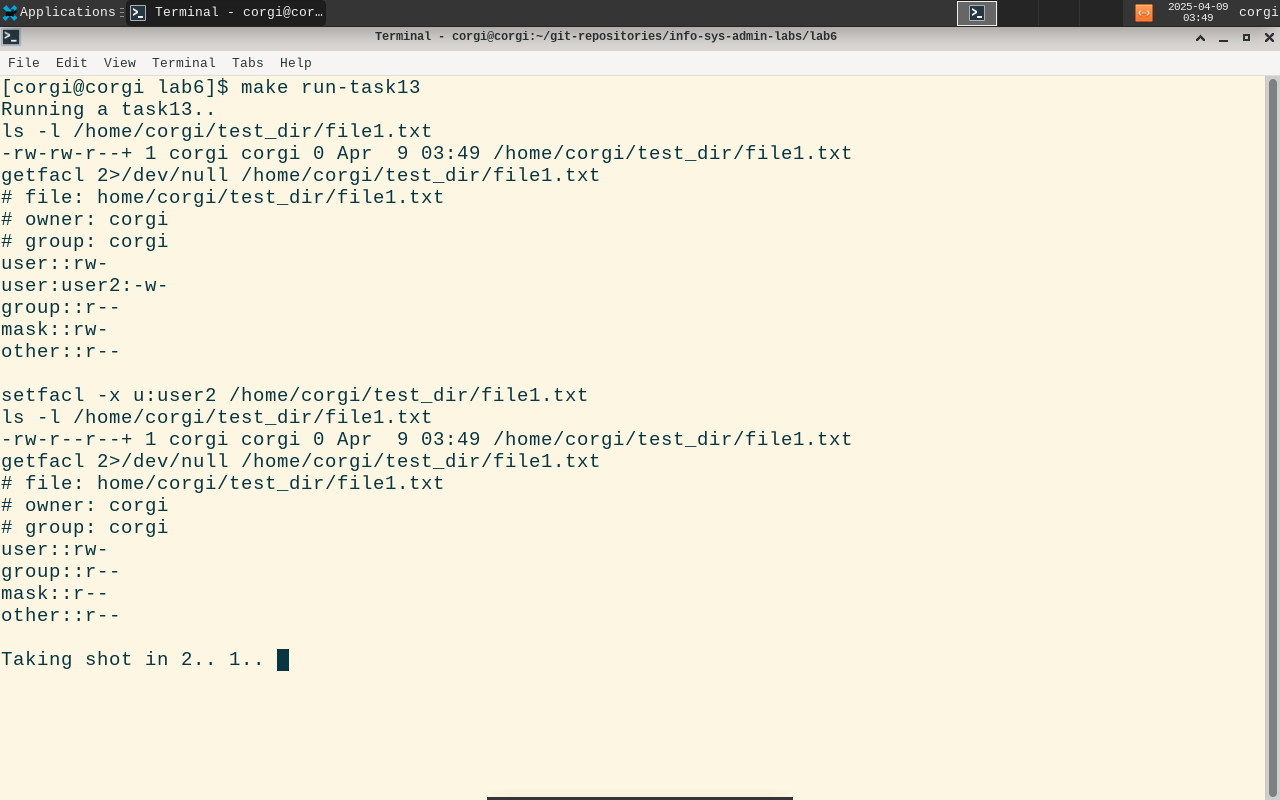
\includegraphics[width=500pt]{task13.png}
			\end{center}

			\subsection*{Задание 14}
			\addcontentsline{toc}{subsection}{Задание 14}
			Создайте под учётной записью \textit{root} одной командой вложенную папку \textit{/tmp/PAPKA2/PAPKA3}. В ней создайте одной командой файл, содержащий десять последних строк файла \textit{/etc/hosts}. Выйдите из-под рута.
			\lstset{style=mystyle}
			\lstinputlisting[language=Bash]{src/task14/main.sh}
			\begin{center}
				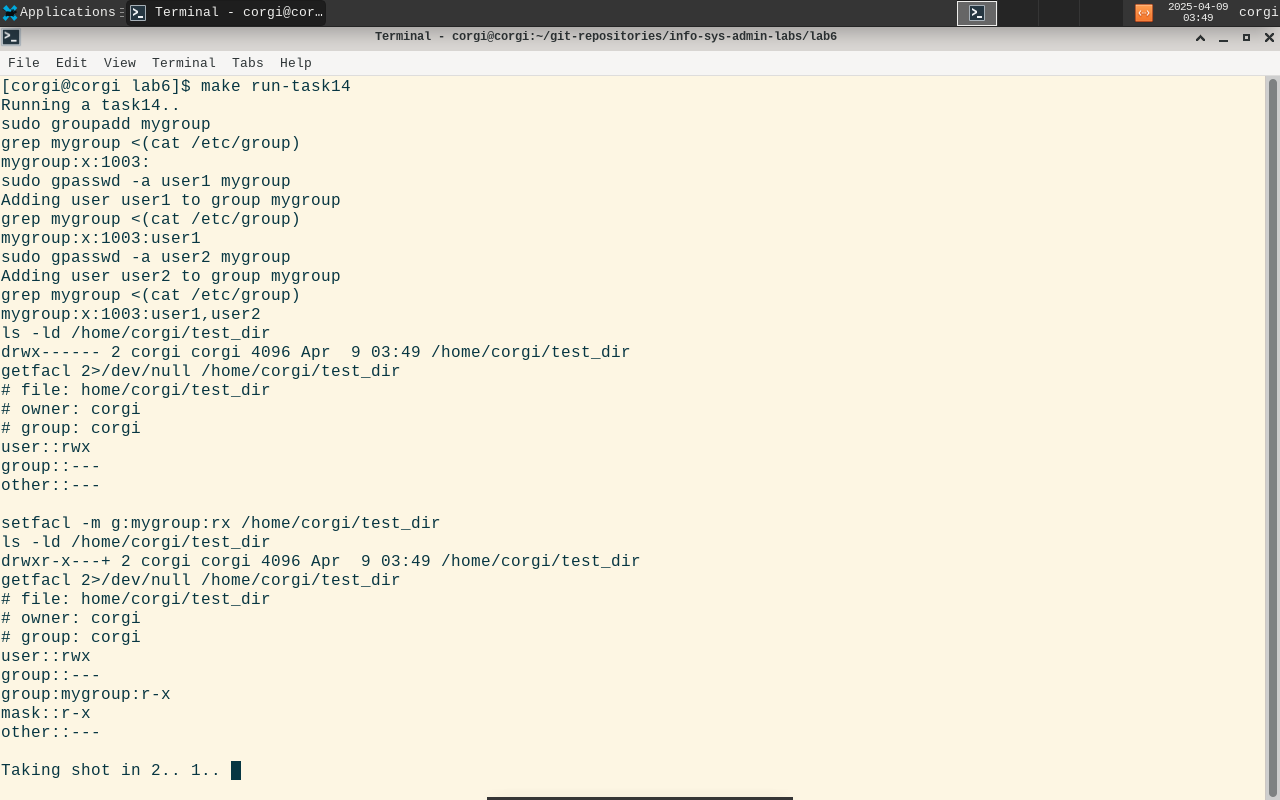
\includegraphics[width=500pt]{task14.png}
			\end{center}

			\subsection*{Задание 15}
			\addcontentsline{toc}{subsection}{Задание 15}
			Под учётной записью \textit{student} создайте в \textit{PAPKA1} файл \textit{4!!4.txt}, содержащий последние десять строк файла \textit{~/.bashrc}. Проверьте, что файл с именем \textit{4!!4.txt} корректно создан - другие имена не принимаются. Добавьте в файл \textit{4!!4.txt}, не затирая прошлые \underline{10} строк, ещё первые \underline{10} строк файла \textit{~/.bashrc}.
			\lstset{style=mystyle}
			\lstinputlisting[language=Bash]{src/task15/main.sh}
			\begin{center}
				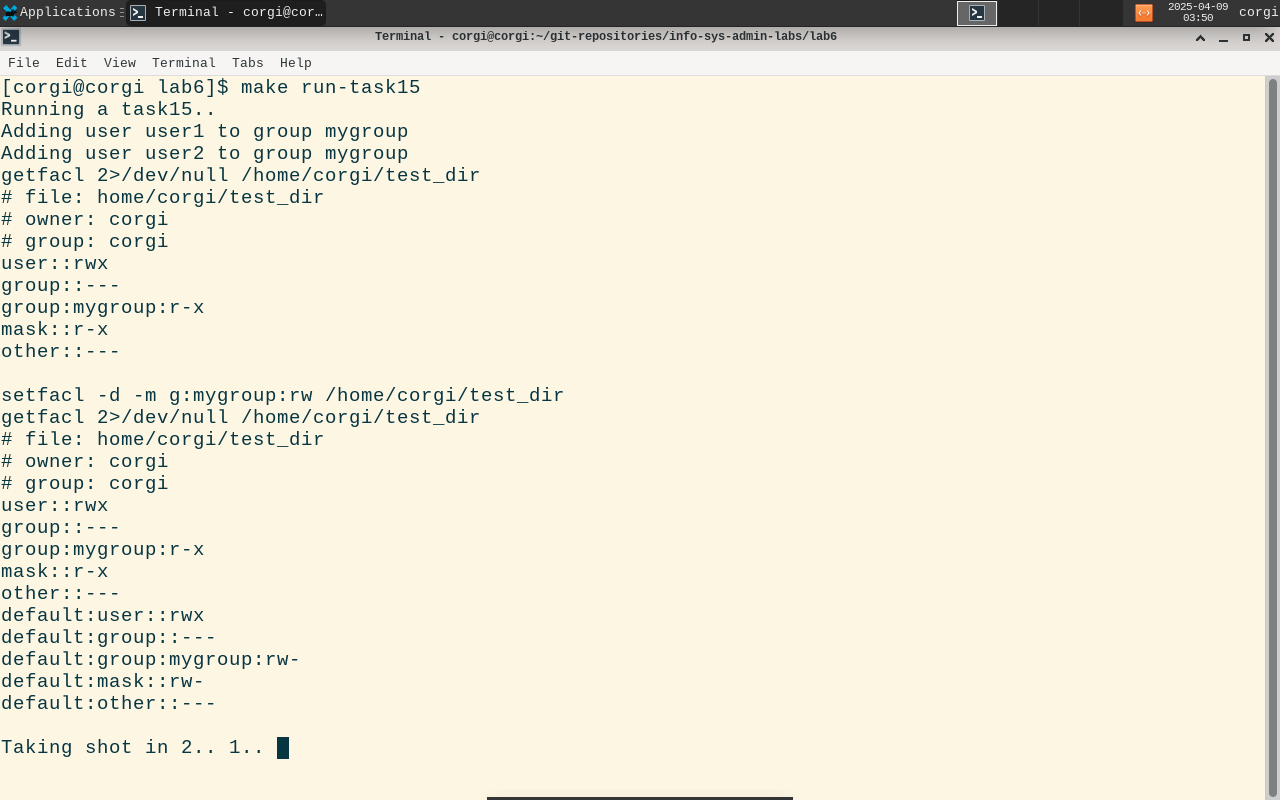
\includegraphics[width=300pt]{task15.png}
			\end{center}

			\subsection*{Задание 16}
			\addcontentsline{toc}{subsection}{Задание 16}
			Под учётной записью \textit{student} попробуйте удалить обе папки командой \textbf{rm} без использования \textbf{опций} команды. Если не получилось, попробуйте удалить их по отдельности. Удалось? Если нет, то укажите причины.
			\lstset{style=mystyle}
			\lstinputlisting[language=Bash]{src/task16/main.sh}
			\begin{center}
				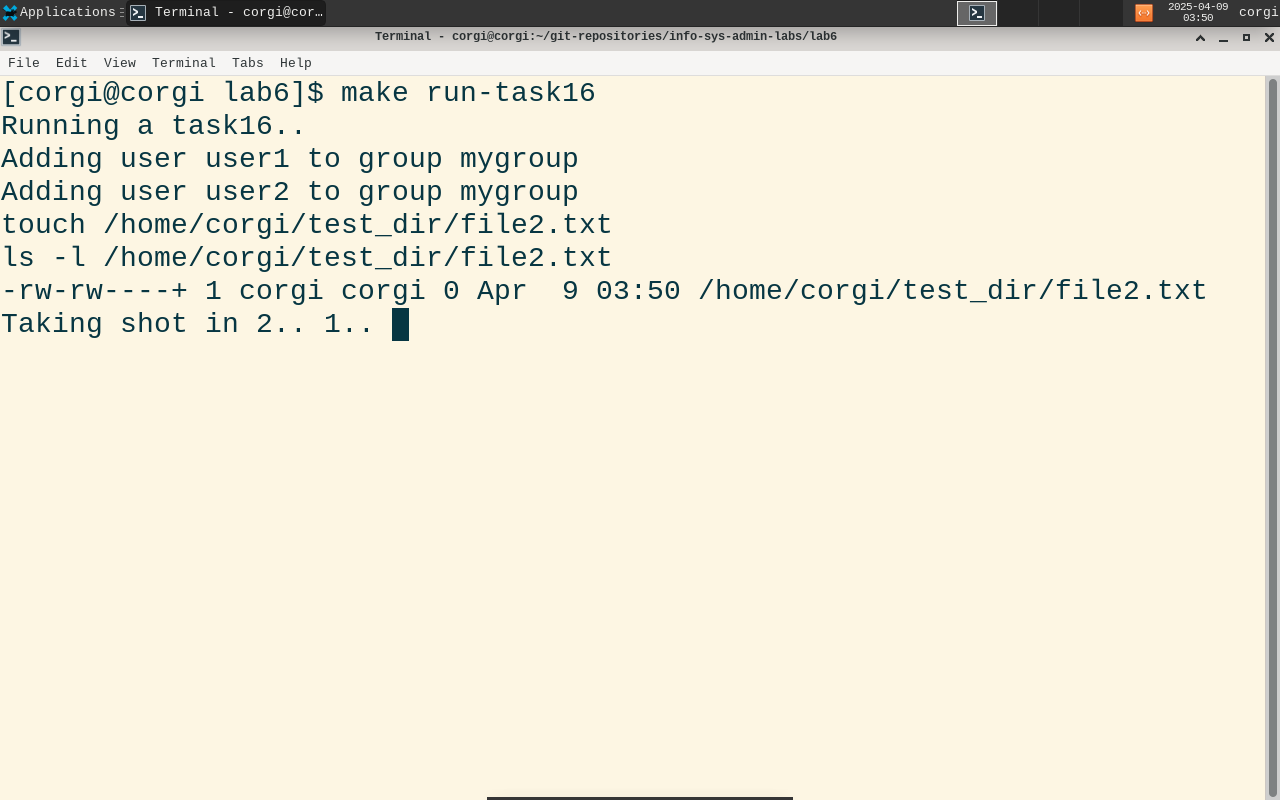
\includegraphics[width=500pt]{task16.png}
			\end{center}

			\subsection*{Задание 17}
			\addcontentsline{toc}{subsection}{Задание 17}
			Изучите файл \textit{~/.bashrc}. Увеличьте максимальную длину файла с историй и максимальное количество строк, выводимых командой \textbf{history} в \underline{10} раз. Сделайте это на постоянной основе (не только, пока запущен данный терминал) - используйте \textbf{export}.
			\lstset{style=mystyle}
			\lstinputlisting[language=Bash]{src/task17/main.sh}
			\begin{center}
				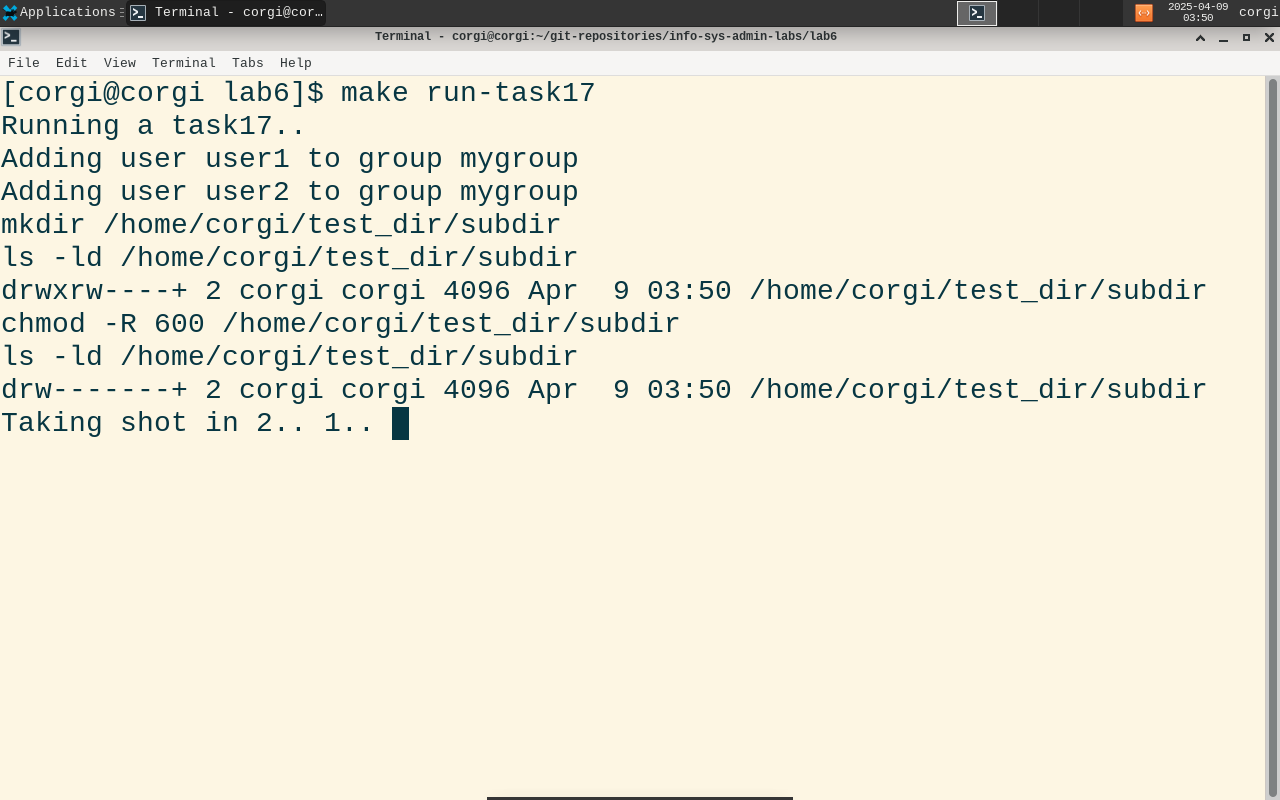
\includegraphics[width=500pt]{task17.png}
			\end{center}

			\subsection*{Задание 18}
			\addcontentsline{toc}{subsection}{Задание 18}
			Выведите содержимое домашней папки в длинном формате вместе со скрытыми файлами сортированной по времени, первыми идёт самые старые файлы и папки. Задание выполнить одной командой \textbf{ls} и её опциями, не использовать команду \textbf{sort}.
			\lstset{style=mystyle}
			\lstinputlisting[language=Bash]{src/task18/main.sh}
			\begin{center}
				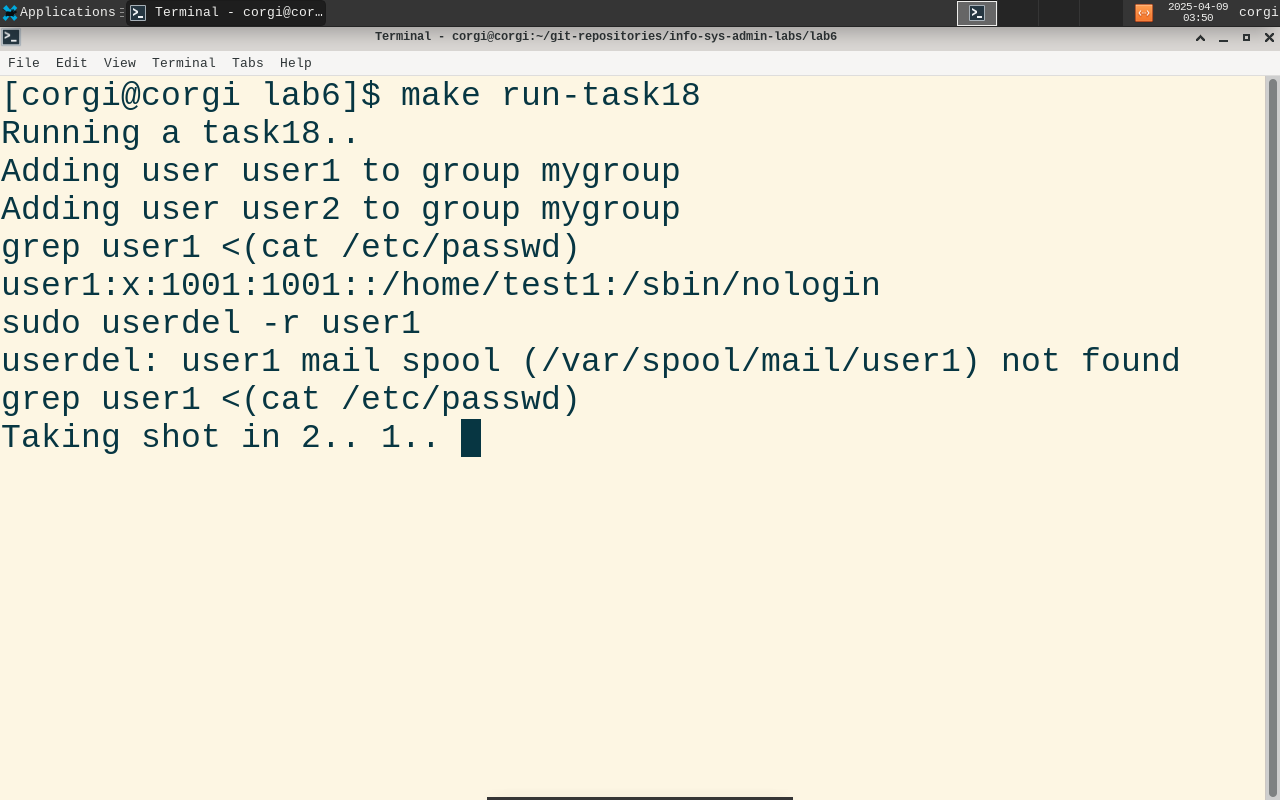
\includegraphics[width=500pt]{task18.png}
			\end{center}

			\subsection*{Задание 19}
			\addcontentsline{toc}{subsection}{Задание 19}
			Создайте в домашней директории папку \textit{bin}, в ней файл \textit{bubble} с правами \underline{744}. В файл добавьте: \par
			\textit{\#!/bin/bash} \par
			\textit{ls} \par
			Запустите её из папки как \textit{./bubble} (добейтесь корректного запуска). \par
			Теперь измените переменную \textit{PATH} системы - внесите запись в \textit{~/.bashrc} - так, чтобы программу \textit{bubble} можно было запустить просто словом \textit{bubble} (не затрите старое значение \textit{\$PATH}, а добавье к ней нужную папку). Молодцы, теперь Вы знаете, зачем нужен \textit{\$PATH}.
			\lstset{style=mystyle}
			\lstinputlisting[language=Bash]{src/task19/main.sh}
			\begin{center}
				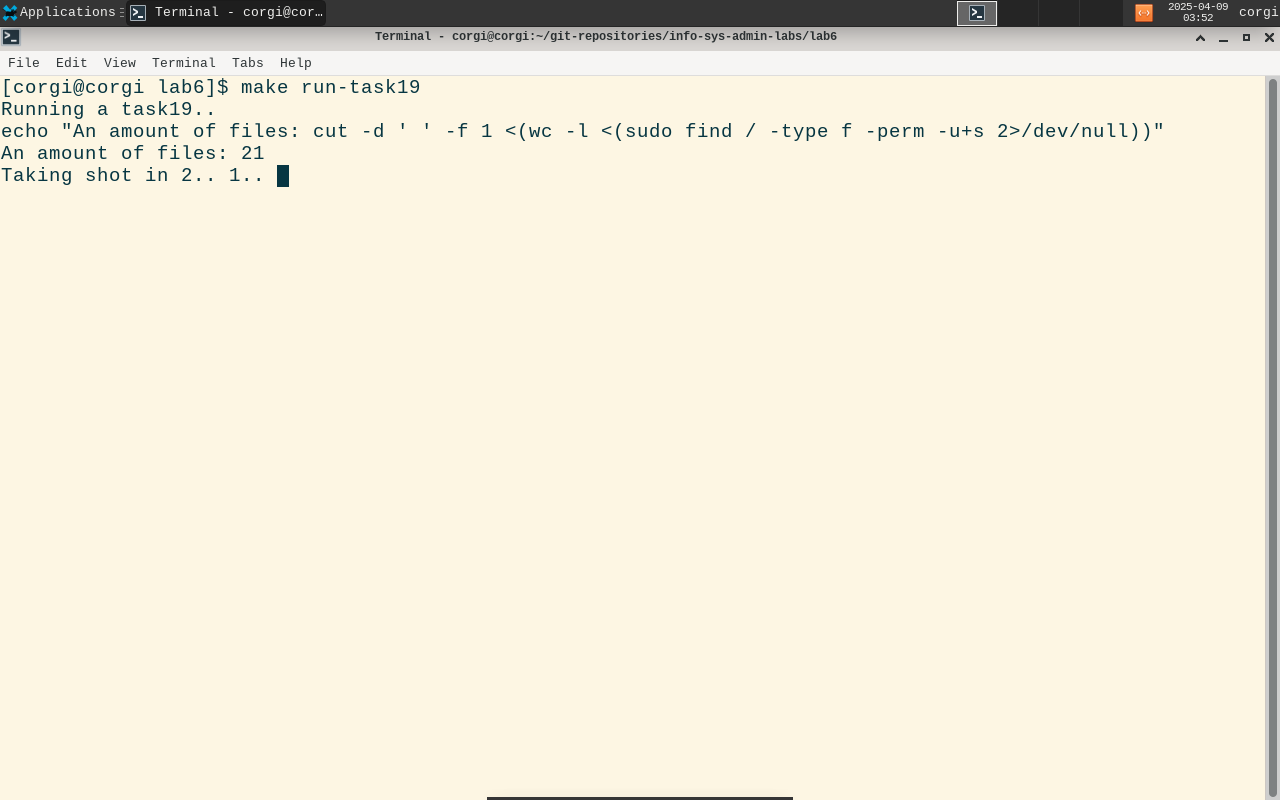
\includegraphics[width=500pt]{task19.png}
			\end{center}

			\subsection*{Задание 20}
			\addcontentsline{toc}{subsection}{Задание 20}
			Заархивируйте три файла в \textit{tarball} со сжатием \textit{bzip2}.
			\lstset{style=mystyle}
			\lstinputlisting[language=Bash]{src/task20/main.sh}
			\begin{center}
				\includegraphics[width=500pt]{task20.png}
			\end{center}

			\subsection*{Задание 21}
			\addcontentsline{toc}{subsection}{Задание 21}
			Теперь создайте папку \textit{PAPKA3} и разархивируйте в неё ваш архив, не перемещая (!) архив внутрь папки.
			\lstset{style=mystyle}
			\lstinputlisting[language=Bash]{src/task21/main.sh}
			\begin{center}
				\includegraphics[width=500pt]{task21.png}
			\end{center}
\end{document}
